% Options for packages loaded elsewhere
\PassOptionsToPackage{unicode}{hyperref}
\PassOptionsToPackage{hyphens}{url}
%
\documentclass[
]{article}
\usepackage{amsmath,amssymb}
\usepackage{lmodern}
\usepackage{iftex}
\ifPDFTeX
  \usepackage[T1]{fontenc}
  \usepackage[utf8]{inputenc}
  \usepackage{textcomp} % provide euro and other symbols
\else % if luatex or xetex
  \usepackage{unicode-math}
  \defaultfontfeatures{Scale=MatchLowercase}
  \defaultfontfeatures[\rmfamily]{Ligatures=TeX,Scale=1}
\fi
% Use upquote if available, for straight quotes in verbatim environments
\IfFileExists{upquote.sty}{\usepackage{upquote}}{}
\IfFileExists{microtype.sty}{% use microtype if available
  \usepackage[]{microtype}
  \UseMicrotypeSet[protrusion]{basicmath} % disable protrusion for tt fonts
}{}
\makeatletter
\@ifundefined{KOMAClassName}{% if non-KOMA class
  \IfFileExists{parskip.sty}{%
    \usepackage{parskip}
  }{% else
    \setlength{\parindent}{0pt}
    \setlength{\parskip}{6pt plus 2pt minus 1pt}}
}{% if KOMA class
  \KOMAoptions{parskip=half}}
\makeatother
\usepackage{xcolor}
\IfFileExists{xurl.sty}{\usepackage{xurl}}{} % add URL line breaks if available
\IfFileExists{bookmark.sty}{\usepackage{bookmark}}{\usepackage{hyperref}}
\hypersetup{
  pdftitle={Dixon Woods},
  pdfauthor={Ted Hillert},
  hidelinks,
  pdfcreator={LaTeX via pandoc}}
\urlstyle{same} % disable monospaced font for URLs
\usepackage[margin=1in]{geometry}
\usepackage{longtable,booktabs,array}
\usepackage{calc} % for calculating minipage widths
% Correct order of tables after \paragraph or \subparagraph
\usepackage{etoolbox}
\makeatletter
\patchcmd\longtable{\par}{\if@noskipsec\mbox{}\fi\par}{}{}
\makeatother
% Allow footnotes in longtable head/foot
\IfFileExists{footnotehyper.sty}{\usepackage{footnotehyper}}{\usepackage{footnote}}
\makesavenoteenv{longtable}
\usepackage{graphicx}
\makeatletter
\def\maxwidth{\ifdim\Gin@nat@width>\linewidth\linewidth\else\Gin@nat@width\fi}
\def\maxheight{\ifdim\Gin@nat@height>\textheight\textheight\else\Gin@nat@height\fi}
\makeatother
% Scale images if necessary, so that they will not overflow the page
% margins by default, and it is still possible to overwrite the defaults
% using explicit options in \includegraphics[width, height, ...]{}
\setkeys{Gin}{width=\maxwidth,height=\maxheight,keepaspectratio}
% Set default figure placement to htbp
\makeatletter
\def\fps@figure{htbp}
\makeatother
\setlength{\emergencystretch}{3em} % prevent overfull lines
\providecommand{\tightlist}{%
  \setlength{\itemsep}{0pt}\setlength{\parskip}{0pt}}
\setcounter{secnumdepth}{-\maxdimen} % remove section numbering
\newlength{\cslhangindent}
\setlength{\cslhangindent}{1.5em}
\newlength{\csllabelwidth}
\setlength{\csllabelwidth}{3em}
\newlength{\cslentryspacingunit} % times entry-spacing
\setlength{\cslentryspacingunit}{\parskip}
\newenvironment{CSLReferences}[2] % #1 hanging-ident, #2 entry spacing
 {% don't indent paragraphs
  \setlength{\parindent}{0pt}
  % turn on hanging indent if param 1 is 1
  \ifodd #1
  \let\oldpar\par
  \def\par{\hangindent=\cslhangindent\oldpar}
  \fi
  % set entry spacing
  \setlength{\parskip}{#2\cslentryspacingunit}
 }%
 {}
\usepackage{calc}
\newcommand{\CSLBlock}[1]{#1\hfill\break}
\newcommand{\CSLLeftMargin}[1]{\parbox[t]{\csllabelwidth}{#1}}
\newcommand{\CSLRightInline}[1]{\parbox[t]{\linewidth - \csllabelwidth}{#1}\break}
\newcommand{\CSLIndent}[1]{\hspace{\cslhangindent}#1}
\ifLuaTeX
  \usepackage{selnolig}  % disable illegal ligatures
\fi

\title{Dixon Woods}
\usepackage{etoolbox}
\makeatletter
\providecommand{\subtitle}[1]{% add subtitle to \maketitle
  \apptocmd{\@title}{\par {\large #1 \par}}{}{}
}
\makeatother
\subtitle{Plant species and descriptions.}
\author{Ted Hillert}
\date{}

\begin{document}
\maketitle

{
\setcounter{tocdepth}{2}
\tableofcontents
}
\hypertarget{galax-unceolata}{%
\section{\texorpdfstring{\emph{Galax unceolata}}{Galax unceolata}}\label{galax-unceolata}}

\begin{figure}

{\centering 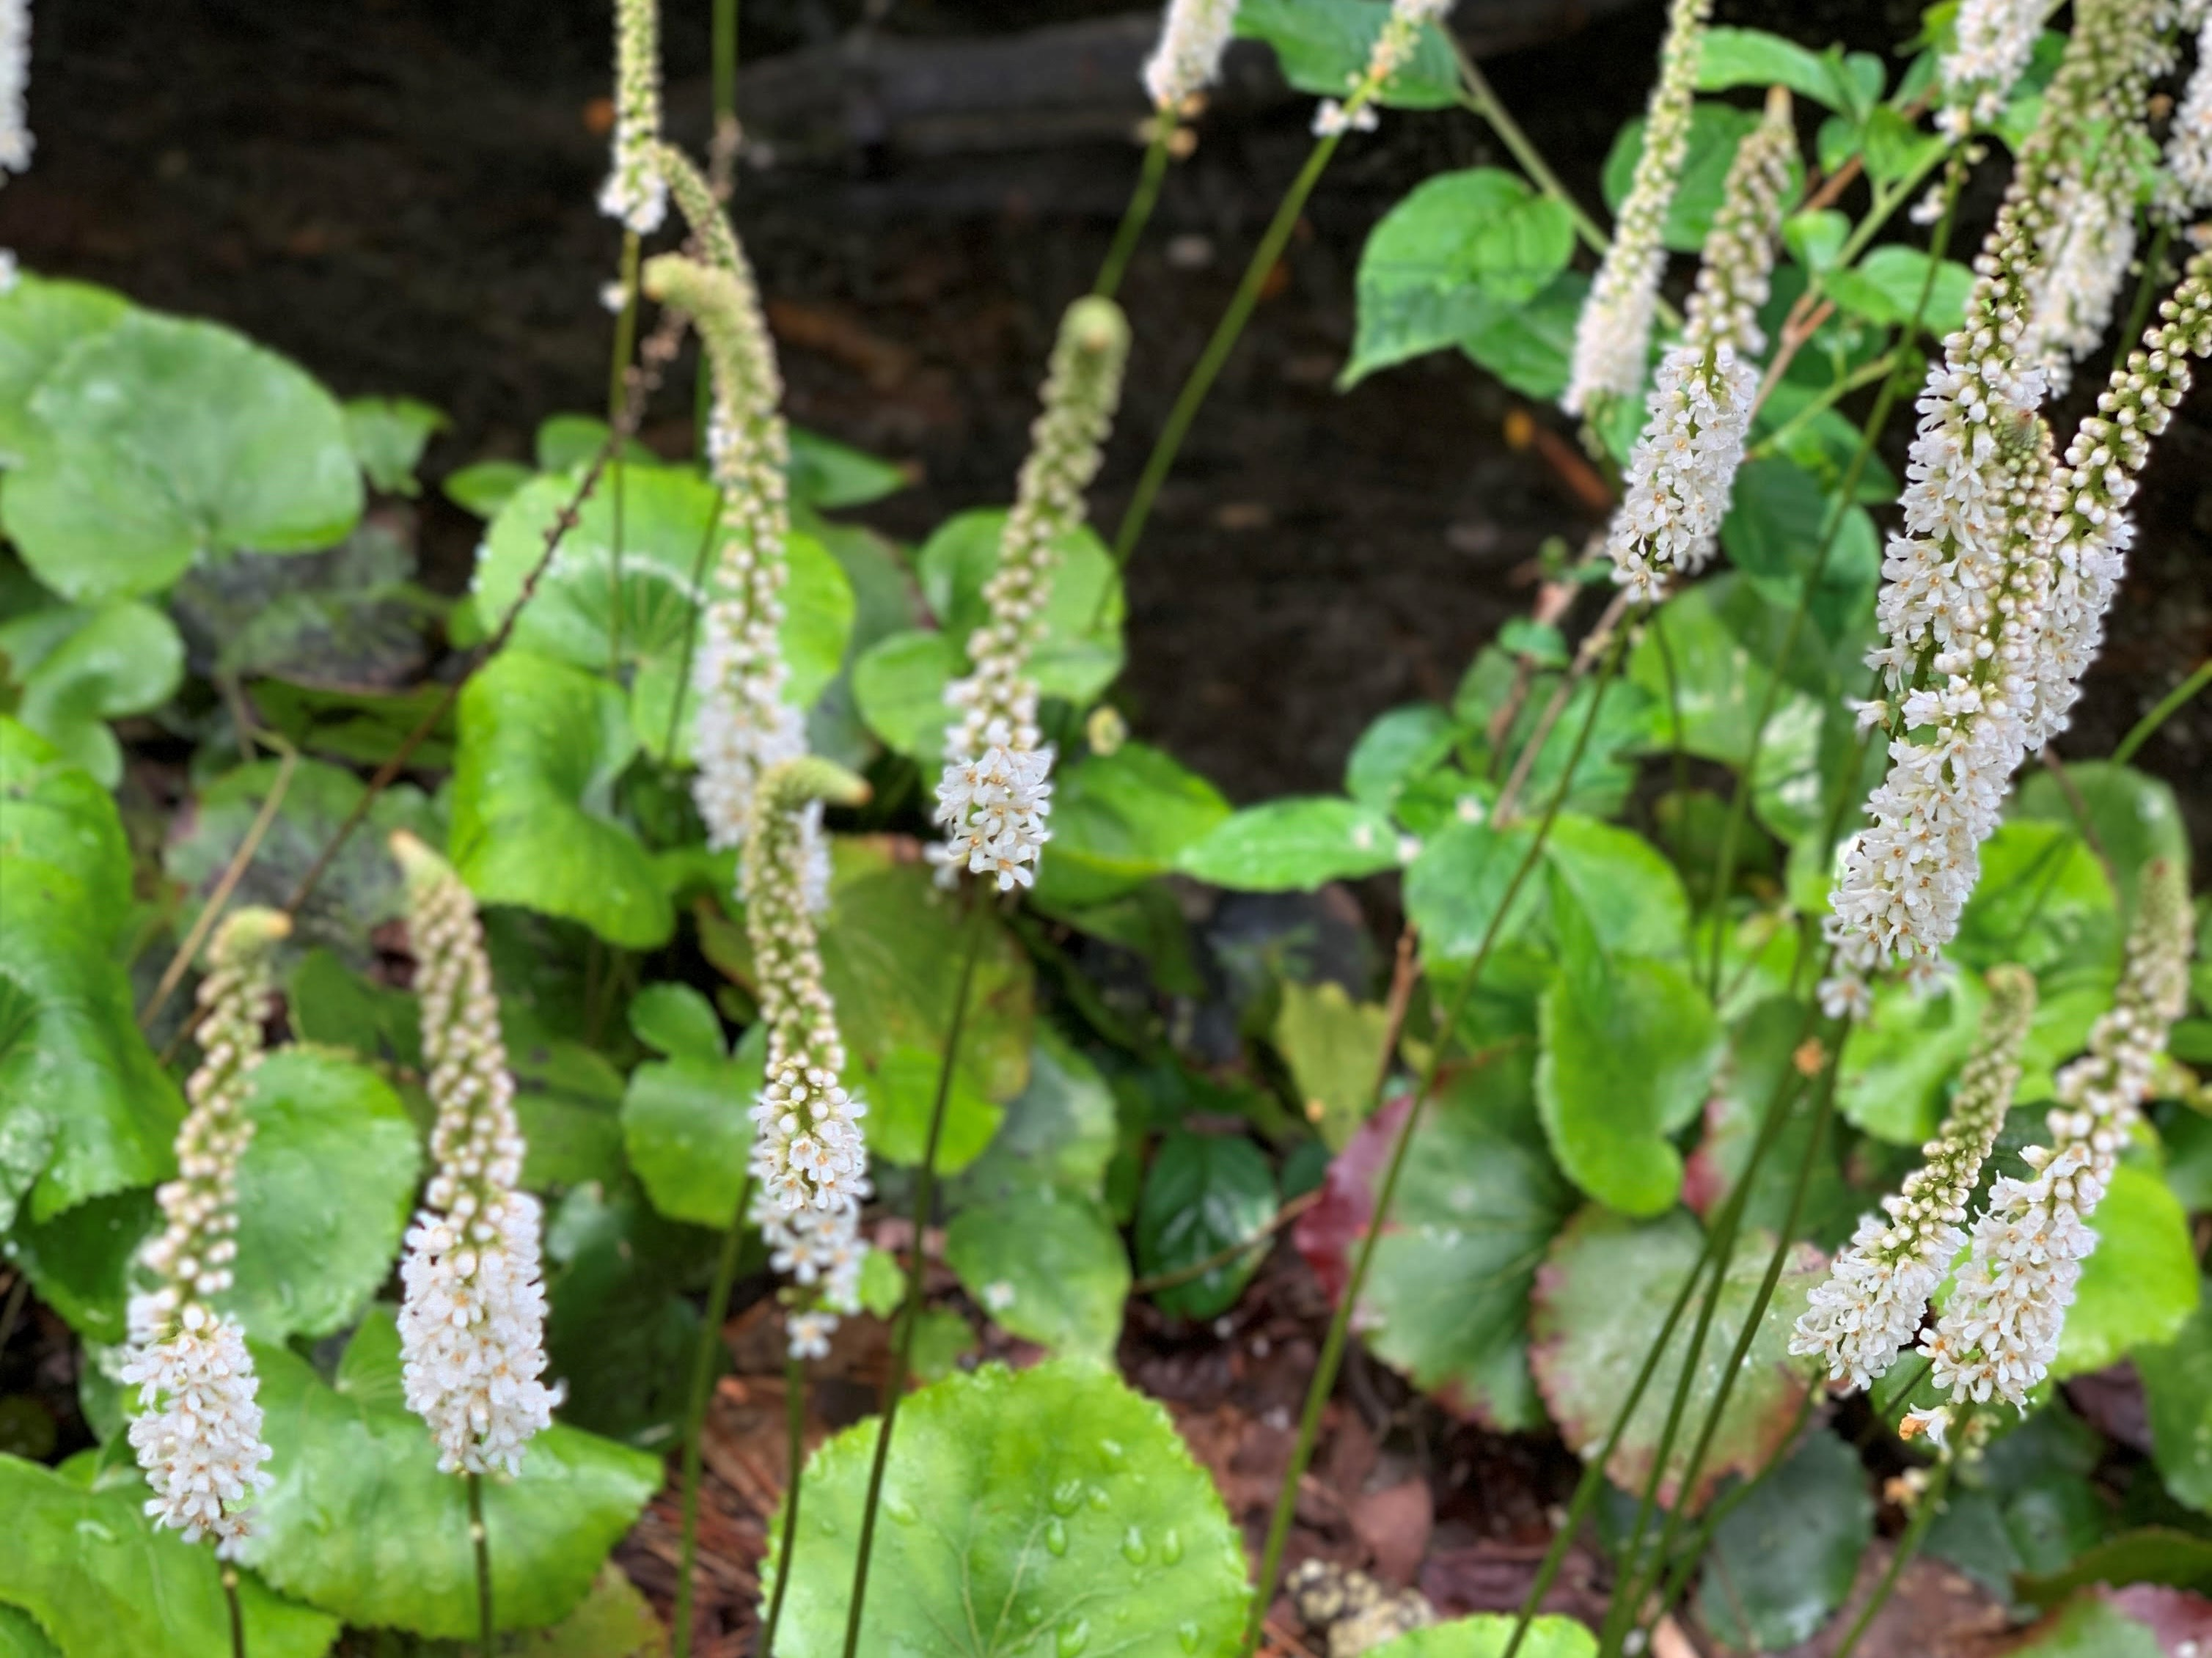
\includegraphics[width=0.5\linewidth]{galax1} 

}

\caption{*Galax unceolata* in bloom.}\label{fig:galax1}
\end{figure}

\hypertarget{common-names-wandflower-wandplant-and-beetleweed.}{%
\subsection{Common names; Wandflower, Wandplant, and Beetleweed.}\label{common-names-wandflower-wandplant-and-beetleweed.}}

\emph{Galax unceolata} is an herbaceous perennial plant native to North America, growing mainly in the Appalachian Mountains up to 1500 meters (4921 feet) in elevation. This species is the sole representative of the plant family Diapensiaceae. This plant grows mainly in the understory of shaded forests and is composed of a rosette of leathery cardioid (heart) shaped. The leaves are serrated along the margin and will turn brown during the winter. Galax flowers in late sprignt to early summer along a single spike-like stem. Each flower is composed of five petals and are white in color. The fruit are capsules containing multiple seeds. The leaves persist throughout the year and are commonly harvested and used as an herbal remedy for cuts and kidney ailments. Although Galax is secure in the Southern Appalachian region, there are concerns about overharvesting particularly in the northern extent of its range.(Predny and Chamberlain 2005)

Further reading: \href{https://www.srs.fs.usda.gov/pubs/gtr/gtr_srs087.pdf}{Galax (\emph{Galax unceolata}): An Annotated Bibliography}

\hypertarget{gaylussacia-spp.}{%
\section{\texorpdfstring{\emph{Gaylussacia spp.}}{Gaylussacia spp.}}\label{gaylussacia-spp.}}

\begin{figure}

{\centering 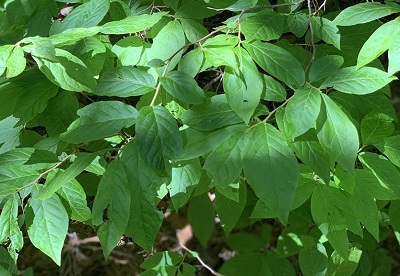
\includegraphics[width=0.5\linewidth]{galuss} 

}

\caption{Foliage of Gaylussacia in a sun fleck.}\label{fig:gayluss}
\end{figure}

\hypertarget{common-names-huckleberry-and-dangleberry}{%
\subsection{Common names; huckleberry and dangleberry}\label{common-names-huckleberry-and-dangleberry}}

\emph{Gaylussacia} is a genus of flowering plants that contains about 50 different species in the Ericaceae family. These deciduous or evergreen shrubs (depending on species) are a common component of oak-heath forests and are native the the Americas. These plant species are used as food by Lepidoptera (butterflies and moths) larvae, including \emph{Coleophora gaylussaciella} which feeds exclusively on these plants. The fruits are edible to humans and are dark purple-black colored berries similar to blueberries (\emph{Vacciunium spp.}). (n.d.)

Further reading: \href{https://www.fs.fed.us/wildflowers/beauty/mycotrophic/monotropa_hypopitys.shtml}{\emph{Gaylussacia baccata} --- black huckleberry}

\hypertarget{monotropa-hypopitys}{%
\section{\texorpdfstring{\emph{Monotropa hypopitys}}{Monotropa hypopitys}}\label{monotropa-hypopitys}}

\begin{figure}

{\centering 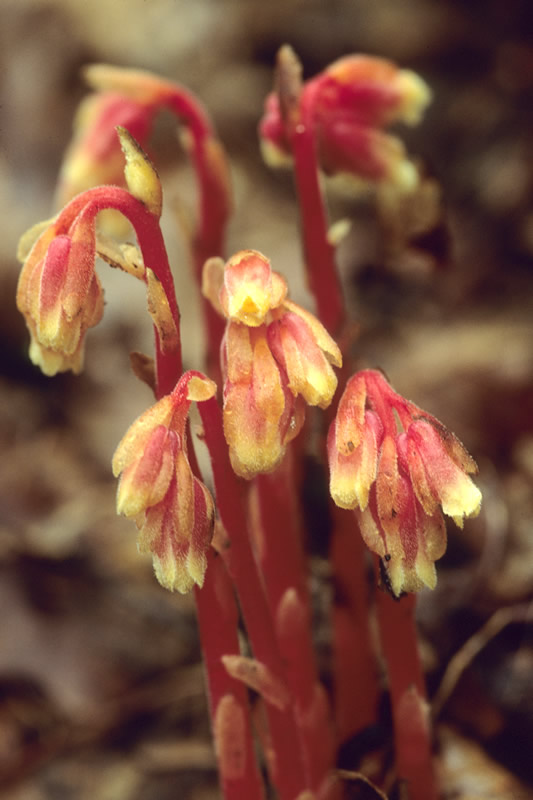
\includegraphics[width=0.5\linewidth]{M hypopitys} 

}

\caption{*Monotropa hypositys* flowers. Photo by Hugh and Carol Nourse.}\label{fig:hypopitys}
\end{figure}

\hypertarget{common-names-dutchmans-pipe-false-beech-drops-pinesap-and-yellow-birds-nest}{%
\subsection{Common names; Dutchman's Pipe, false beech-drops, pinesap, and yellow bird's-nest}\label{common-names-dutchmans-pipe-false-beech-drops-pinesap-and-yellow-birds-nest}}

\emph{Monotropa hypopitys} is an herbaceous perennial plant that grows to height between 10 and 35 cm. In North America, \emph{M hypopitys} flowers from May to October in mature, moist, shaded forests often under pine trees (``hypo'' - under, ``pitys'' - pine). Each plant produces a single unbranched inflorescence that are analogous (similar in function but different evolution) to adventitious roots that appear pale yellowish-white to red-tinged. This is because the plant is parasitic in nature and obtains its nutrients from photosynthetic trees connected via fungal mycorrhizal networks. The leaves, or bracts, are scale-like and cover most of the inflorescence. The flowers of this plant emerge as pendants and become erect when the fruit matures. Plants that flower in the summer tend to be yellow and sparsely hairy, while those blooming in autumn tend to be red and densely hairy. It is proposed that the summer blooms are self-pollinating. (USFS n.d.a)

Further reading: \href{https://www.fs.fed.us/wildflowers/beauty/mycotrophic/monotropa_hypopitys.shtml}{\emph{Monotropa hypopitys} - Pinesap, Dutchman's Pipe}

\hypertarget{monotropa-uniflora}{%
\section{\texorpdfstring{\emph{Monotropa uniflora}}{Monotropa uniflora}}\label{monotropa-uniflora}}

\begin{figure}

{\centering 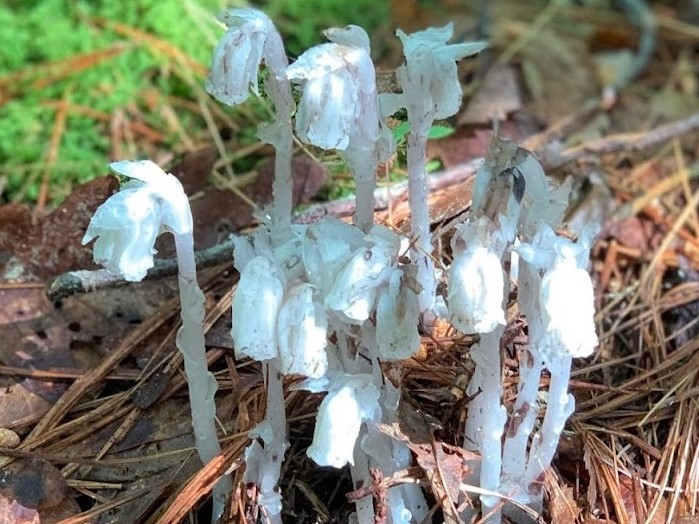
\includegraphics[width=0.5\linewidth]{M uniflora} 

}

\caption{*Monotropa uniflora* flowers.}\label{fig:uniflora}
\end{figure}

\hypertarget{common-names-indian-pipe-and-ghost-plant}{%
\subsection{Common names; Indian Pipe and Ghost Plant}\label{common-names-indian-pipe-and-ghost-plant}}

\emph{Monotropa uniflora} is an uncommon perennial wildflower that grows to height between 10 and 30 cm. \emph{M uniflora} blooms in early summer through early autumn in mature, moist, shaded forests. This plant is entirely translucent white while sometimes appearing in a pale pinkish-hue. This is because the plant is parasitic in nature and obtains its nutrients from photosynthetic trees (commonly Beech; \emph{Fagus sp.}) connected via fungal mycorrhizal networks. The leaves that arise directly from the peduncle (flower stalk) are scale-like and can be flecked black. As the name suggests (\emph{M uniflora}), this plant has single-flowers that emerge as pendants (pointed downward). Once the flower matures it erects perpendicular to the stalk. The fruits are capsules with seeds that release through slits along the length of the capsule. The flowers can persist following seed dispersal however the flesh may become desiccated and look brown or black. (USFS n.d.b)

Further reading: \href{https://www.fs.fed.us/wildflowers/beauty/mycotrophic/monotropa_uniflora.shtml}{\emph{Monotropa uniflora} - Ghost Plant, Indian Pipe}

\hypertarget{pinus-rigida}{%
\section{\texorpdfstring{\emph{Pinus rigida}}{Pinus rigida}}\label{pinus-rigida}}

\begin{figure}

{\centering 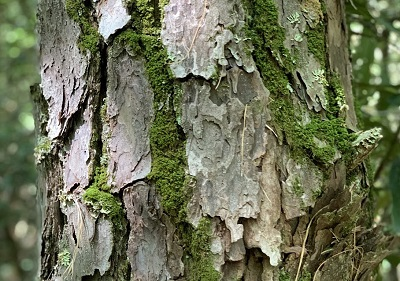
\includegraphics[width=0.5\linewidth]{p rigida bark} 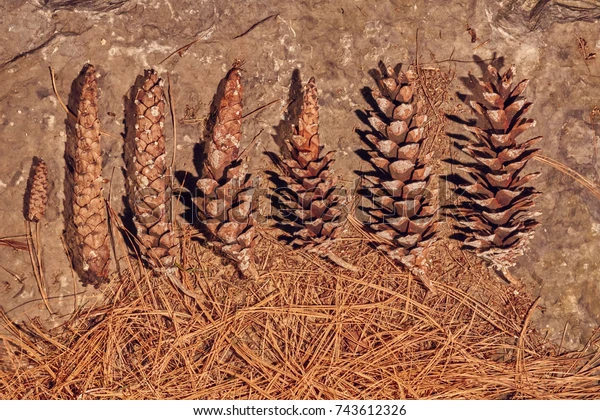
\includegraphics[width=0.5\linewidth]{pitch pine cones} 

}

\caption{*Pinus rigida* bark (Left). Cone life stages (Right), photo courtesy of C. N. Elliot.}\label{fig:rigida}
\end{figure}

\hypertarget{common-names-pitch-pine}{%
\subsection{Common names; Pitch pine}\label{common-names-pitch-pine}}

\emph{Pinus rigida} is mainly found in the southern areas of the northeastern United States. These trees are found in environments other species may find unfavorable (i.e.~acidic, sandy, and low nutrient soils). The needles of this tree come in fascicles of three, grow to a length of 6-13 cm (2.25-5 inches), and are often slightly twisted. The cones of this tree are serotinous, meaning, they need to be exposed to an internal temperature of 100°C/212°F and can survive external temperatures as high as 421°C/790°F. The trunks of pitch pine are usually straight and covered in large, thick, irregular plates of bark. The thick bark provides an adaptation against fire by insulating the sensitive cambium layer from heat. It also has a remarkable regenerative ability, should it be damaged by cuts or fire, it can resprout using epicormic shoots (grow from the bark). Pitch pine is a pioneer species in abandoned agricultural or pasture land and is replaced by hardwoods, spruce, or other pines in the absence of disturbance. (Gucker 2007)

Further reading: \href{https://www.fs.fed.us/database/feis/plants/tree/pinrig/all.html\#Cone\%20survival\%20and\%20seedling\%20establishment:}{\emph{Pinus rigida}}

\hypertarget{references}{%
\section*{References}\label{references}}
\addcontentsline{toc}{section}{References}

\hypertarget{refs}{}
\begin{CSLReferences}{1}{0}
\leavevmode\vadjust pre{\hypertarget{ref-gaylussacia}{}}%
\href{https://plants.ces.ncsu.edu/plants/gaylussacia-baccata/}{(n.d.). }.

\leavevmode\vadjust pre{\hypertarget{ref-rigida}{}}%
Gucker, C. L. 2007. \href{https://www.fs.fed.us/database/feis/plants/tree/pinrig/all.html\#Cone\%20survival\%20and\%20seedling\%20establishment:}{Pinus rigida}.

\leavevmode\vadjust pre{\hypertarget{ref-galax}{}}%
Predny, M. L., and J. L. Chamberlain. 2005. \href{https://www.srs.fs.usda.gov/pubs/gtr/gtr_srs087.pdf}{Galax (galax urceolata): An annotated bibliography}. U.S. Department of Agriculture, Forest Service, Southern Research Station.

\leavevmode\vadjust pre{\hypertarget{ref-hypopitys}{}}%
\href{https://www.fs.fed.us/wildflowers/beauty/mycotrophic/monotropa_hypopitys.shtml}{USFS. (n.d.a). }.

\leavevmode\vadjust pre{\hypertarget{ref-uniflora}{}}%
\href{https://www.fs.fed.us/wildflowers/beauty/mycotrophic/monotropa_uniflora.shtml}{USFS. (n.d.b). }.

\end{CSLReferences}

\end{document}
